\documentclass[11pt, letterpaper]{report}
\usepackage{geometry}
\usepackage{graphicx, subfigure}
\usepackage[spanish]{babel}
\usepackage{xcolor}
\definecolor{darkblue}{rgb}{0, 0, 0.5}
\usepackage[colorlinks=true,linkcolor=black,anchorcolor=black,citecolor=darkblue,filecolor=black,menucolor=black,runcolor=black,urlcolor=darkblue]{hyperref}
\usepackage[utf8]{inputenc}
\usepackage[T1]{fontenc} 
\usepackage{setspace}
\geometry{lmargin=3cm, rmargin=3cm, tmargin=2.65cm, bmargin=3cm}
\usepackage[pages=some]{background}
\usepackage{natbib}
\usepackage{sectsty}
\usepackage{amssymb,amsmath}

\backgroundsetup{
	scale=1,
	angle=0,
	opacity=1,
	color=black,
	hshift=-159,
	contents={\includegraphics[width=0.48\paperwidth,height=\paperheight]{images/portada.png}}
}


\begin{document}
	\begin{titlepage}
	\begin{minipage}[t]{0.48\textwidth}
		\BgThispage
		\parbox{\textwidth}{}
	\end{minipage}
	\begin{minipage}[t]{0.55\textwidth}
			\parbox{\textwidth}{
				\includegraphics[width=.8\textwidth]{images/logo.png}\\[0.5cm]
				\centering\textsc{Facultad de Ciencias Naturales y Exactas}\\[0.2cm]
				\centering\textsc{Departamento de Ciencia de la Computación}\\[2.2cm]
				\textbf{\LARGE Trabajo de Diploma en\\[-.1cm]Opción al Título de\\[-.1cm]Licenciado en Ciencia de la\\[-.1cm]Computación\\[2.2cm]}
				\Large  \textbf{Título}:\\
				\fontsize{18pt}{20pt}\selectfont Aprendizaje Profundo para el Perfilado de Usuarios en Redes Sociales\\
				\vspace{10mm}
				\begin{tabular}{rp{0.7\textwidth}}
					{\Large \bf Autor:} & {\Large Roberto Labadie Tamyao} \\[.5cm]
					{\Large \bf Tutores:} & {\Large Dr. Daniel Castro Castro} \\[.5cm]
					& {\Large M.Sc. Reynier Ortega Bueno} \\[.5cm]
				\end{tabular}
				
				\vspace{10mm}
				{\Large \textbf{Curso 2020-2021}}
			}
	\end{minipage}
	\end{titlepage}
	
	\pagenumbering{roman}
	\thispagestyle{empty} 	
	\chapterfont{\flushright}
	\renewcommand{\contentsname}{Contenido} \tableofcontents
	\renewcommand{\listfigurename}{Lista de Figuras}
	\renewcommand{\tablename}{Tabla}

	\listoffigures
	
%	\renewcommand{\listtablename}{Lista de Tablas}
%	\listoftables
	\pagenumbering{arabic}
\addcontentsline{toc}{chapter}{Introducción}
\chapter*{Introducción}
Internet se define como la interconexión mundial de redes individuales operadas por el gobierno, la industria, el mundo académico y las partes privadas. En cuestión de muy pocos años, Internet se consolidó como una plataforma muy poderosa que ha cambiado para siempre la forma de comunicarse.  Esta manera tan simple y accesible de compartir datos, ha propiciado un desplazamiento de los entes sociales hacia el uso casi exclusivo de este medio.
\\
Un rol fundamental dentro de este universo comunicativo lo juegan las redes sociales donde, de acuerdo al sitio DataReportal\footnote{\url{https://datareportal.com/}}, a finales de 2020 existían más de 3.8 mil millones de usuarios de los 4.5 mil millones de personas conectadas a Internet, lo cual implica un crecimiento desmedido de la cantidad de datos multimodales que se generan a diario.
\\
El mundo del Big Data \citep{Riahi2018BigDA} en el cual nos sumerge este hecho, reporta una situación beneficiosa para el desarrollo de procesos sociales en cuanto a la cantidad de información brindada por los usuarios. 
Estos procesos van desde estudios de marketing, donde la retroalimentación a partir de opiniones permiten dirigir de manera efectiva la promoción hacia grupos sociales específicos, hasta aplicaciones en el área de la \ac{hci}, donde el conocimiento de las características físicas y psicológicas de los individuos permite personalizar la interfaz de comunicación. Sin embargo, un cúmulo de información tan significativo se hace imposible de tratar en un espacio de tiempo razonable, a menos que se haga de manera automatizada.
\\
Diversos estudios se han dirigido al diseño de métodos para manejar la información digital y realizar inferencias a partir de la misma, a la vez que han contribuido al desarrollo en ramas como el \ac{nlp}, \ac{tm} y \ac{cv} en el área de la \ac{ai}.
\\ 
Dentro de la Minería de Textos, la tarea de \ac{ap} \citep{Rosso2019,article} se encarga específicamente de realizar un análisis de la información textual elaborada por una persona, que permita establecer atributos y patrones de comportamiento para caracterizarla en cuanto a sexo, rango de edad o rasgos personales (e.g si la persona es extrovertida o no, ideología política). Para el AP el hecho de que la información recuperada de estos textos varíe enormemente en términos de su formato, aun cuando proviene de la misma persona, sumado a que las secuencias textuales constituyen información digital no estructurada, hacen desafiante el proceso de analizarla y clasificarla automáticamente. 
\\
Inicialmente este tipo de tareas se desarrollaban sobre contenido generado en textos formales, periódicos, cartas o revistas; sin embargo, determinar el perfil de una persona mediante el análisis de su cuenta en una red social ha tomado un gran auge en los últimos años \citep{rangel:2018,rangel:2019,f6032ffbacb14369b7a45d1ba9bd0b8c}.
 Las redes sociales, además de haber logrado acelerar la comunicación entre las personas, así como reunir varias formas de pensamiento individual en un mismo espacio, se han convertido en un medio donde se desarrollan procesos negativos tales como la divulgación de discursos de odio \citep{rangel2021profiling}, de \textit{bullying} o de noticias falsas \citep{rangel:2020}, introduciendo así nuevos retos al AP, con tareas que involucran la detección de elementos altamente subjetivos como la ofensa, la toxicidad en el lenguaje y otros patrones psicológicos de comunicación que hacen más complejo el perfilado en relación a otras tareas.  
\\
 La mayor parte de los avances en el desarrollo de sistemas de AP ha sentado sus bases dentro del ambiente académico, reuniendo estudios tanto de la Ciencia de la Computación como de la Lingüística. Algunas de las campañas de evaluación más importantes donde se han compartido tareas de este tipo son \ac{pan}\footnote{https://pan.webis.de/} y \ac{evalita}\footnote{http://www.evalita.it/}, los que se han dirigido últimamente al análisis del genero textual de micro-blogging  con un enfoque multilingüe como el existente en medios sociales como Twitter.\footnote{https://twitter.com/}
\\
Tradicionalmente se han empleado dos tipos de acercamiento que han probado empíricamente ser efectivos para tratar el AP en redes sociales: los \textit{basados en estilo}  y los \textit{basados en contenido}. Las propuestas basadas en estilo se refieren al hecho de analizar cómo los autores se expresan cuando escriben; en cambio las basadas en contenido se apoyan en el área temática del texto analizado. La mayor contribución de varios trabajos parte de la selección de atributos que permitan medir el \textit{estilo autor} y el \textit{contenido} simultáneamente mediante el empleo de métodos de \ac{ml}.
\\
Un procedimiento crítico en este tipo de propuestas es la selección de rasgos para representar vectorialmente los textos. Aquí puede ser introducida información ruidosa afectando el desempeño de los modelos o pueden ser eliminados elementos que ayuden a dicho modelo a discernir la pertenencia de un objeto a una clase u otra para el caso de tareas de clasificación o estimar un valor para las tareas de regresión.
\\
\\
En los últimos años, dentro del Machine Learning, se ha hecho popular el \acl{dl} en las áreas de \ac{cv} y \ac{nlp}, estableciendo nuevos estados del arte en la mayoría de sus tareas \citep{electronics8030292}. Este auge estuvo condicionado por las capacidades de procesamiento de las nuevas computadoras y la cantidad de datos disponibles. Los modelos de \ac{dl} han mostrado una gran habilidad para aprender representaciones de rasgos (\textit{features}) con un alto nivel de abstracción. Estas representaciones capturan elementos que son posiblemente omitidos mediante la extracción manual de \textit{features} y que facilitan el proceso de inferencia de los propios modelos de \ac{dl} y de los métodos más tradicionales de \ac{ml}. 
\\
Dentro del \ac{ap} también se ha introducido el \acl{dl} con resultados alentadores. Sin embargo, la mayoría de los modelos alcanzan mejores resultados al analizar la tarea a la que se orienta el perfilado cuando se emplean para clasificar mensajes individuales en lugar del perfil completo, e.g., se desempeñan mejor en la tarea de detección de odio en un tweet que en la detección de un perfil que tiende a usar un discurso de odio. 
\\
Por otro lado, las necesidades que cubren las tareas de AP incluyen la no sensibilidad de los sistemas ante la variación del idioma en el que la persona publique un mensaje o escriba una carta, es por ello que urge la extensión de los modelos de AI propuestos al esquema multilingüe que predomina en redes sociales como Twitter. \\Este trabajo de tesis se enmarca en el perfilado de autores en redes sociales empleando técnicas de Aprendizaje Profundo para el modelado y la clasificación de los perfiles, teniendo en cuenta el enfoque multilingüe propio de este medio. 

%\addcontentsline{toc}{section}{Problemática}
\section*{Problemática}
La mayoría de los trabajos existentes que emplean DL para resolver tareas de perfilado de autores en redes sociales, tanto tradicionales (e.g., determinar rango de edades, sexo, etc.) como las más recientes (e.g. detección de divulgadores de discursos de odio o de noticias falsas en redes sociales) ven afectado su desempeño al tratar con las secuencias muy largas que se pueden generar al analizar un perfil completo de manera simultánea, en vez de mensaje a mensaje. La pérdida de información en este tipo de secuencias, en términos de relaciones a largo plazo que presentan las estructuras sintácticas del lenguaje, es la causa fundamental de esta dificultad. Por esta razón sería conveniente dividir el problema de ``clasificar un perfil'' en subproblemas y construir una arquitectura modular en la que primero se modele el perfil y luego este sea clasificado.
\\
Por otro lado, en Cuba existe un limitado tratamiento y aplicación de este tipo de métodos automatizados para llevar acabo tareas de impacto como las mencionadas, ya sea en el área forense o empresarial.

%\addcontentsline{toc}{section}{Objetivos}
\section*{Objetivos}
\subsection*{Objetivo General}
Diseñar una arquitectura modular basada en Aprendizaje Profundo para resolver la tarea de Perfilado de Autores en redes sociales teniendo en cuenta un enfoque multilingüe.
\subsection*{Objetivos Específicos}
\begin{enumerate}
	\item Diseñar una arquitectura que capture rasgos abstractos que permitan clasificar un perfil de usuario de una red social, atendiendo tanto a tareas relacionadas con características demográficas de los autores como con aspectos psicológicos de los mismos.
	\item Extender la arquitectura propuesta a un enfoque multilingüe de las tareas evaluadas.
	\item Evaluar y analizar el empleo de arquitecturas modulares basadas en DL sobre colecciones de datos propuestas en tareas de AP, compartidas en la plataforma PAN (2019, 2020, 2021).
\end{enumerate}

%\addcontentsline{toc}{section}{Hipótesis}
\section*{Idea a defender}
Dividir el proceso de clasificación de un perfil dentro de una tarea en: (i) codificar los mensajes individualmente y (ii) modelar-clasificar el perfil, puede ayudar a prevenir la pérdida de información generada del análisis de largas secuencias. Esto sumado a la capacidad de representar la información no estructurada de los métodos de DL puede influir positivamente en la precisión de las predicciones.  Además, proponer un modelo lo suficientemente robusto, podría incentivar el empleo de esos métodos automatizados  de AP en nuestro país.

\section*{Estructura del Trabajo}
Este trabajo está estructurado en tres capítulos además del introductorio y una última sección en la que se describen las conclusiones de las modelaciones y se proponen  caminos a seguir para trabajos futuros. Cada uno de los capítulos se listan a continuación: 

%%Poner la reerencia de cada capitulo cuando este listo
\begin{itemize}
	\item En el Capítulo 1 se describen de manera breve métodos del estado del arte, así como conceptos básicos relacionados con el Machine Learning, necesarios para la comprensión de este trabajo.
	\item El Capítulo 2 describe cada uno de los submodelos de la arquitectura propuesta para enfrentar la tarea de perfilado de autores.
	\item En el Capítulo 3 se exponen las tareas, así como sus respectivos \textit{corpus} de datos con los que se evaluará la arquitectura, además de  los experimentos realizados en el proceso de ajuste de cada unos de los modelos sobre los idiomas estudiados. 
\end{itemize}
. 
	
\chapter{Fundamentos}

\section{Estado del Arte}\label{SOTA}

El Procesamiento del Lenguaje Natural, como cualquier tarea llevada a cabo por un algoritmo de Machine Learning, se basa en el análisis de un conjunto de rasgos del objeto a procesar, con la finalidad de realizar inferencias que permitan al sistema computarizado interactuar con el usuario.
\\
Para la tarea de  AP no es diferente, por lo que la mayoría de los trabajos se dirigen al desarrollo de una efectiva selección de rasgos, estableciéndose dos categorías fundamentales; los rasgos de estilo y los de contenido.  
\\
El análisis de estilo se enfoca en la detección de rasgos estilísticos del autor que sean lo suficientemente invariantes a lo largo de los pasajes escritos, pero que varíen de un autor a otro. Ejemplos de estos podrían ser la longitud media de las oraciones o la cantidad esperada de símbolos de puntuación, emoticones, preposiciones o  adverbios que usa en un párrafo.
\\
Por otra parte el análisis de contenido se enfoca en la información contextual siguiendo la misma estrategia del análisis de estilo, i.e., llevar información estadística de la presencia de determinado conjunto de palabras o estructuras gramaticales. Este tipo de rasgos incluye el uso de n-gramas de palabras y caracteres, \textit{slang words}\footnote{ \textit{slang} se refiere a un lenguaje muy informal empleado por un grupo particular de personas.}, Bolsas de Palabras (\textit{Bag of Words} BoW) \citep{DBLP:conf/clef/Pizarro19,DBLP:conf/clef/Valencia-Valencia19}, palabras concluyentes (e.g., finalmente, para concluir, en conclusión, etc.)  y lexicones de palabras.
Dentro de este último método para categorizar palabras, el más empleado es el sistema \textit{Linguistic Inquiry and WordCount LIWC} \citep{pennebaker2015development} el cual contiene alrededor de 70 diccionarios de lexicones divididos en categorías como; Preocupaciones personales (\textit{Personal Concerns}), Discurso informal (\textit{Informal Speech}), Impulsos (\textit{Drives}) y necesidades fundamentales (\textit{Basics Needs}), etc.
\\\\
Estos dos grupos de rasgos, de estilo y contenido, son ortogonales puesto que los rasgos que se tienen en cuenta para capturar estilo, son precisamente aquellos que son independientes del tópico, por lo cual se ha hecho habitual el uso de enfoques que los combinen a ambos. Por otro lado el empleo de elementos contextuales implica introducir en el proceso de clasificación un sesgo hacia una clase que este más representada por determinado tema, e.g., según \citep{schler2006effects} estos rasgos pueden facilitar la determinación del sexo del autor ya que por ejemplo los hombres mayormente tienden a hablar de política y noticias, mientras que las mujeres se muestran más interesadas por la moda, fiestas y prendas de vestir; sin embargo es posible encontrar una mujer que regularmente postee tweets relacionados con deportes o automóviles, luego este perfil sería potencialmente mal clasificado por un modelo de AP basado en rasgos de contenido.
\\
La mayoría de los trabajos de Machine Learning han usado métodos de clasificación tradicionales como Regresión Logística (Logistic Regression LR) \citep{DBLP:conf/clef/Valencia-Valencia19}, Máquina de Vectores de Soporte (\textit{Support Vector Machines} SVM) \citep{DBLP:conf/clef/Pizarro19}  y Bosques Aleatorios (\textit{Random Forest} RF) \citep{DBLP:conf/clef/Johansson19} combinando conjuntos de rasgos que responden a estas clasificaciones.
\\
\\
 Con la introducción del Deep Learning en el NLP esta tendencia a la extracción manual de rasgos de tipo estadístico ha sido desplazada por el aprendizaje de rasgos abstractos que representan a las estructuras gramaticales atendiendo no solamente a su significado semántico como elementos aislados del texto, sino que tienen en cuenta además el contexto en el que son empleados, facilitando la comprensión y clasificación de los textos tanto a los propios modelos de DL como a los tradicionales de ML. Este tipo de enfoques se basan fundamentalmente en el uso de \textit{embeddings} preentrenados con distintas estrategias \citep{DBLP:conf/clef/JooH19,DBLP:conf/clef/Lopez-Santillan19}, principalmente Word2Vec \citep{DBLP:conf/nips/MikolovSCCD13}, Glove\citep{pennington2014glove} y Fasttext\citep{bojanowski2016enriching}.
 \\
 Las Redes Neuronales Artificiales como mecanismos de aprendizaje y clasificación, por su parte han logrado un desempeño superior a los métodos tradicionales de ML en muchas tareas de NLP, teniendo en cuenta que aprenden a decidir que elemento del texto tomar como rasgo significativo a la hora de modelar los objetos. Esquemas especializados en análisis de secuencias, como las Redes Neuronales Recurrentes (RNN) \citep{DBLP:conf/clef/DiasP19,bakhteev:2020} y las arquitecturas \textit{Transformers} (Transformadoras) \citep{iyer:2020,baruah:2020} se han empleado satisfactoriamente para el perfilado de autores en los últimos años, pero también se ha extendido el uso de arquitecturas diseñadas inicialmente para el tratamiento de otro tipo de información estructurada como las imágenes, tal es el caso de las Redes Neuronales Convolucionales (CNN) \citep{DBLP:conf/clef/PetrikC19,DBLP:conf/clef/Lopez-Santillan19}.
 \\
 \\
 En los últimos años dentro de PAN se han propuesto tareas de perfilado que van desde la predicción de sexo y variedad del idioma  hasta la detección de perfiles manejados por bots y perfiles que tienden a difundir discursos de odio en el medio social. En la mayoría de estas tareas los trabajos con un mejor desempeño se han enmarcado en técnicas tradicionales de ML, tal es el caso de \citep{basile:2017} en la tarea \textit{Gender and Language Variety Identification in Twitter at} PAN 2017, quien empleó rasgos a partir de una medida no estándar de frecuencia de términos sobre unigrama de palabras y n-gramas de caracteres para entrenar una SVM y \citep{martinc:2017}  que combinó n-gramas de palabras, caracteres y Elementos del Discurso (\textit{Part of Speech} POS), además de información de sentimientos relacionada con el uso de emojis, conteo de elongación de caracteres, con otros rasgos de estilo para modelar el perfil y entrenar un Regresor Logístico. 
 \\
 La tarea \textit{Bots and Gender Profiling in Twitter at} PAN 2019 consistente en determinar si una cuenta de Twitter pertenece a un bot o a un humano y en el segundo caso, inferir el sexo; \citep{DBLP:conf/clef/Pizarro19} obtuvo la mejor precisión con una SVM combinando representaciones de los tweets mediante \textit{tf-idf} de n-gramas de palabras y caracteres. De igual forma \citep{DBLP:conf/clef/Johansson19} trató de dar solución a la tarea empleando ML con Random Forest y rasgos de estilo como logitud de los tweets, número de letras mayúsculas, URLs, menciones, cantidad de RTs, así como rasgos de contenido, específicamente ocurrencia de términos y etiquetas de POS.
 \\ 
 Nuevamente en PAN 2020 en la tarea \textit{Profiling Fake News Spreaders on Twitter}, para detectar divulgadores de noticias falsas, \citep{pizarro:2020} se basó en la combinación de vectores de \textit{tf-idf} de n-gramas de palabras y caracteres para representar los tweets y clasificar los perfiles con una SVM. Mientras el modelo propuesto por \citep{buda:2020} consistió en un Regresor Logístico que combina las predicciones de cinco submodelos: (i) n-gramas con Regresor Logístico,(ii) n-gramas con SVM, (iii) n-gramas con Random Forest, (iv) n-gramas con XGBoost y (v) XGBoost con features de estilo.
 \\
Diversos modelos de DL empleando las arquitecturas citadas anteriormente (e.g., RNN y CNN) han sido propuestos a lo largo de estas competiciones, aunque ninguno de ellos mostró una precisión superior a la de los métodos tradicionales de ML. Sin embargo en la tarea \textit{Profiling Hate Speech Spreaders on Twitter at} PAN 2021, el modelo con mejor desempeño, propuesto por \citep{sinno:2021} empleó una Red Neuronal Convolucional sobre la representación de los perfiles con \textit{embeddings} de palabras. 
\\\\
Uno de los mayores problemas con los enfoques predominantes es que los rasgos extraídos son muy dependientes del contexto lo cual puede crear una alta sensibilidad de los modelos ante datos que no correspondan a los corpus con los que han sido refinados sus parámetros o como ya hemos expuesto tengan un sesgo hacia alguna clase. Por ejemplo \citep{Newman2008GenderDI} expone que las mujeres tienden a usar emoticones con mayor regularidad que los hombres, lo contrario de lo concluido por \citep{Schwartz2013PersonalityGA}. Esto nos sugiere que métodos tan rigurosamente refinados como lo son los dependientes de rasgos manualmente extraídos tienen una menor robustez ante arquitecturas \textit{End-to-End} como las de Deep Learing.

\section{Marco Teórico}

En este epígrafe se realiza un acercamiento hacia los temas y arquitecturas de Machine Learning necesarios para la comprensión de los modelos propuestos en el trabajo.

\subsection{LSTM: Long Short-Term Memory Neural Networks}

	Las LSTM son un tipo de Redes Neuronales Recurrentes, las cuales están especializadas en el análisis de datos secuenciales. 
	Las RNNs tienen una unidad principal (la unidad recurrente) la cual explora la secuencia de datos de entrada de un elemento a la vez, ya sea de izquierda a derecha o viceversa. Al analizar un elemento para la determinación de su estado oculto, se comparte la información capturada en pasos anteriores del recorriendo. Esto es, sea $h_{t-1}$ el último estado oculto computado, $x_t \in \Re^d$ el $t-esimo$ elemento de la secuencia de entrada y $f$ una función de no linealidad. El estado oculto actual, se define como:
	\begin{equation}
		h_t = f(W_xx_t + W_hh_{t-1} + b_h)
		\label{rrn_form}
	\end{equation}
	Donde $W_x \in Re^{n_u\times d}$ y $W_h \in Re^{n_u\times n_u}$ son matrices de parámetros y $b_h \in R^{n_u}$ el término de sesgo (\textit{bias}), con $n_u$ el número de neuronas y $d$ la dimensión de los vectores que representan a los elementos de la secuencia.
	De esta forma la arquitectura aprende a considerar la información que tiene determinada influencia sobre el elemento de la secuencia que se analiza en cada paso como se muestra en la \figurename~\ref{rnn}, lo que le otorga una especie de ``memoria''.
	\begin{figure}[!thb]
		\begin{center}
			\includegraphics[width=250pt]{images/rnn.png}
		\end{center}
		\caption[Red Neuronal Recurrente]{Red Neuronal Recurrente sobre la secuencia $X_t$. \citep{agarwala2017music}}
		\label{rnn}
	\end{figure}
	\\
	Sin embargo, debido a que en las RNNs durante el proceso de \textit{backpropagation}, en el que se ajustan los parámetros de la red, cada neurona en la unidad principal calcula su gradiente para un paso del recorrido de la secuencia con respecto a su estado en el paso posterior, mediante la ley de la cadena, ocurre un decrecimiento exponencial de los valores de las derivadas parciales conocido como \textit{gradient vanishing}, lo que hace que los parámetros a penas se actualicen y se dificulte el aprendizaje de relaciones a largo plazo, de aquí su ``Short-Term Memory''.
	\\
	Esta limitación es lo que las LSTM tratan de solucionar introduciendo compuertas que deciden que información preservar u ``olvidar'' de los estados previos en el recorrido por la secuencia de la siguiente forma:
	\\
	Sean $W_f, W_i, W_o \in \Re^{n_u\times d}$ y $U_f, U_i, U_o \in \Re^{n_u\times n_u}$ las matrices de parámetros de la compuerta de ``olvidar '', entrada y salida respectivamente y $b_f, b_i, b_o \in \Re^{n_u}$ sus respectivos términos de bias:
	
	\begin{equation}
		\begin{split}
		i_{t} &= \sigma(W_i x_t + U_i  h_{t-1} + b_i)\\
		o_{t} &= \sigma(W_o x_t + U_o h_{t-1} + b_o)\\
		f_t &= \sigma(W_{f} x_t + U_f   h_{t-1} + b_f) 
		\end{split}
		\label{lstm_gates}
	\end{equation}
	\\
	Una codificación potencial $\hat{c}_t$ considerando el elemento $x_t$ de la secuencia y el estado previo $h_{t-1}$ esta dado por:
	\begin{equation}
		\hat{c}_{t} = \sigma(W_cx_t + U_c h_{t-1} + b_c)
		\label{lstm_pu}
	\end{equation}
	\\
	Donde $W_c\in\Re^{n_u\times d}$, $U_c\in\Re^{n_u\times n_u}$ y  $b_c\in\Re^{n_u}$. Luego la codificación $x_t$ teniendo en cuenta la codificación del elemento anterior y $h_t$ quedan definidos por:
	 \begin{equation}
	 	\begin{split}
	 		c_{t} &= f_tc_{t-1} +i_t\tanh(\hat{c}_{t})\\
	 		h_t &= o_t\tanh(c_t)
	 	\end{split}
	 	\label{lstm_hstate}
	 \end{equation}
 
 
\subsection{Redes Neuronales Convolucionales sobre secuencias}
	
	La arquitectura de una CNN \citep{lecun1998gradient} sobre una secuencia de texto es capaz de capturar dependencias temporales a corto plazo mediante filtros unidimensional que analizan n-gramas de palabras o caracteres y cuyos parámetros son compartidos durante cada paso de manera similar a las LSTM.
	\\
	Esto es, sea $X \in \Re^{l\times d}$ la secuencia de entrada de longitud $l$ donde cada elemento es un vector $d-dimensional$, $F_k$ el conjunto de filtros con ventana $k$ de una capa convolucional, cada uno de los ${F_k}_i \in \Re^{k\times d}$ son inicializados de manera independiente y de la misma forma aprenden a capturar relaciones a corto plazo  dentro en $X$. La operación convolución (\textit{conv-op}) transforma a $X$ en una nueva secuencia $X' \in \Re^{(l - k) \times n_f}$ donde $n_f = |F_k|$ de la siguiente forma:
	
	\begin{equation}
		X'_{ij} = \sum X_{[i:i+k]} * {F_k}_j ~~~ para ~~~ j \in [0, F_k-1], \;i \in [0, l-k]
	\end{equation}
	\\
	Como se puede observar en la \figurename~\ref{cnn}:
	\begin{figure}[!thb]
		\begin{center}
			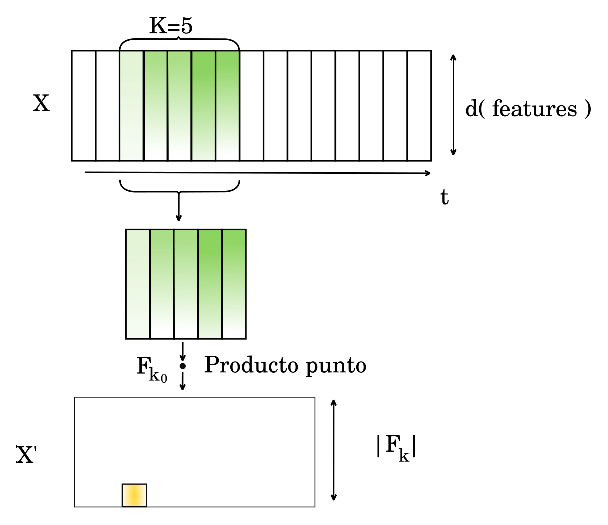
\includegraphics[width=250pt]{images/cnn.eps}
		\end{center}
		\caption[Operación Convolución. CNN]{Operación convolución sobre $X$ con filtros de tamaño de ventana k. }
		\label{cnn}
	\end{figure}
	\\
	Vinculada a la \textit{conv-op} en este tipo de arquitectura se suele emplear además una capa de \textit{pooling}, en la cual se combinan los valores de elementos en una vecindad para reducir la dimensionalidad de la secuencia o se seleccionan los valores más importantes de dicha vecindad, esta operación de \textit{pooling} con una ventana de tamaño $k$  sobre una secuencia $X$ esta definida por:
	\begin{equation}
		X'_i = f(X_{[i:i+k]}) ~~ para ~~~  \;i \in [0, l-k]
	\end{equation}
	\\
	Donde $f$ es la función de \textit{pooling}, regularmente empleadas las funciones $Max$ o $Avg$.
		
\subsection{Mecanismos de Atención}\label{atencion}

	Los mecanismos de atención, son técnicas de procesamiento de las entradas de una arquitectura o de algún resultado intermedio que permiten a la red prestar mas ``atención'' a elementos específicos de una secuencia o establecer la importancia relativa sobre un elemento del resto. En la práctica, la atención permite a las redes neuronales aproximarse al mecanismo de atención visual que utilizan los humanos.

	\subsubsection{Self-Attention}
	
		Sea $x_t$ la representación del $t-esimo$ elemento de la secuencia, una capa de \textit{self-attention} (auto-atención), captura en una matriz $A$ cuan similar es $x_t$ con sus vecinos. Específicamente $\alpha_{t, t'} \in A$ expresa la relación de $x_t$ con $x_t'$ y de manera similar al de una red recurrente este valor se calcula como:
		\begin{equation}
			\begin{split}
				g_{t, t'} &= \tanh(W_{x}x_t + W_{x{t'}}x_{t'} + b_g)\\
				a_{t, t'} &= \sigma({W_{a}g_{t, t'} + b_{a}}) 
			\end{split}
		\end{equation}
		\\
		Donde $\sigma$ es la función sigmoide, $W_{x}, W_{x{t'}} \in \Re^{n_u \times d} $ son las matrices de parámetros encargadas de codificar la información de $x \text{ y } x'$ para expresar su compatibilidad, $W_a \in \Re^{n_u \times n_u}$ la matriz de parámetros correspondiente a su combinación no lineal y $b_g \text{ y } b_a$ los correspondientes términos de bias.
		\\
		A partir de $A$ el estado correspondiente al vector $x_t$, $\hat{x}_t$ está dado por la suma ponderada de sus elementos vecinos $x'_t$:
		
		\begin{equation} \label{attention}
			\hat{x}_t = \sum \limits_{i=0} a_{t,t'}x_{t'}
		\end{equation}
		\\
		Luego $\hat{x}_t$ expresa cuan atendido debe ser $x_t$ condicionado por el contexto de su vecindad.
	
	\subsubsection{Scaled Dot-Product Attention}
		
		El mecanismo \textit{Scaled Dot-Product Attention} (Atención con Producto-Punto Escalado) primero se mapea cada elemento de la secuencia con tres representaciones (\textit{query} y un par \textit{key-value}) para calcular el índice de compatibilidad entre cada par de elementos. Luego, para cada $x_t$ es evaluada su compatibilidad con respecto a cada uno de los  elementos vecinos relacionando su \textit{query} ($q_t$) con las \textit{keys} de los vecinos ($k_{t'}$), estos valores de compatibilidad son escalados y normalizados con la función $softmax$ y empleados para ponderar los vectores de \textit{value} ($v_t$). Finalmente la representación de $\hat{x}_t$ es calculada como la suma ponderada de los $v_t$. En forma matricial queda expresado como:
		
		\begin{equation}
			Attention(Q, V, K) = softmax(\frac{Q\times K^T}{\sqrt{d_k}})\times V
			\label{dotP-att}
		\end{equation} \\
		Donde $Q, K \in \Re^{n\times d_k} \text{ y } V \in \Re^{n\times d_v} $ son el resultado del producto de las matrices de parámetros de \textit{query}, \textit{key} y \textit{value} con los elementos de la secuencia respectivamente, por tanto en la fila $t$ contienen el mapeo del elemento $x_t$ y  $d_k,d_v$ corresponden a la dimensionalidad de las vectores de \textit{key} y \textit{value} respectivamente.
		
\subsection{Transformers}

	La arquitectura Transformer (\figurename~\ref{transformer}) basada en mecanismos de atención, específicamente \textit{multihead attention} \citep{vaswani2017attention}, está diseñada para tratar problemas de \textit{machine translation} y la conforman dos módulos, el primero conocido como \textit{Encoder} (Codificador) es alimentado con una secuencia textual y se encarga de encontrar una codificación para cada elemento teniendo en cuenta la información de su contexto. El segundo módulo, \textit{Decoder} produce los elementos de una nueva secuencia en el modelado de lenguaje, haciéndolo de uno a la vez y teniendo en cuenta los elementos generados anteriormente y las codificaciones obtenidas por el Encoder de la secuencia de entrada.
	\\
	La principal ventaja de las Transformers con respecto a las arquitecturas secuenciales más tradicionales, e.g., GRU y LSTM es que en vez de analizar la información textual en una dirección, esta toma en consideración la entrada completa relacionando cada elemento con el contexto de su vecindad simultáneamente lo cual evita el problema de ``memoria'' a corto plazo de las RNN.  Sin embargo pudiera parecer que existe una pérdida de la percepción del tiempo al analizarlo todo a la vez, es por esto que ademas de representar el texto con un \textit{embedding} de palabras, se tiene en cuenta un \textit{encoding} de posición. 
	\begin{figure}[!thb]
		\begin{center}
			\includegraphics[width=.5\linewidth, height=.5\textheight]{images/transformer.png}
		\end{center}
		\caption[Arquitectura Transformer]{Arquitectura Transformer. Módulo Izquierdo, Codificador. Módulo Derecho, Decodificador. \citep{vaswani2017attention} }
		\label{transformer}
	\end{figure}
	\\
	En la \figurename~\ref{transformer} se observan cada uno de los módulos los cuales se apilan ($N_x$), i.e., antes de que el Decoder reciba la informacion codificada de la secuencia de entrada, esta transita por una serie de bloques codificadores haciendo uso de una red residual para prevenir cualquier pérdida de la información.
	\\
	Dentro de la mayoría de las tareas de NLP este tipo de modelo ha alcanzado nuevos estados del arte simplemente haciendo \textit{transfer learning} del modulo de Encoder hacia la tarea específica. Este módulo es entrenado en dos tareas: (i) predecir palabras enmascaradas de la secuencia; (ii) dadas dos oraciones, predecir si una está a continuación de la otra en el texto, lo cual hace que el modelo llegue a ``entender'' el funcionamiento del lenguaje y sea relativamente fácil de entrenar sobre otras tareas como el análisis de sentimientos. Para esta última tarea, dado el par de oraciones como una secuencia, se añade un \textit{token} [CLS] al inicio del cual su estado oculto se toma para realizar la clasificación y otro [SEP] al final de cada oración. 
	
\subsection{Redes Neuronales Convolucionales en Grafos}
	
	La principal diferencia entre las CNNs y las Redes Neuronales Convolucionales en Grafos (\textit{Graph Convolutional Neural Nets }GNN) es que las primeras están diseñadas especialmente para tratar datos regularmente estructurados (Euclideanos), mientras que las GNN son su versión generalizada capaz de extraer información en datos donde no existe una relación de orden entre un nodo y otro y las conexiones entre cada uno de ellos es variable (datos irregulares o datos estructurados no Euclideanos), estas dos propiedades son totalmente opuestas a las relaciones que existen entre los píxeles de una imagen (\figurename~\ref{euclidian-non}).
	\begin{figure}[!thb]
		\centering
		\subfigure[Datos Estructurados Euclideanos]{\includegraphics[width=0.35\textwidth]{images/cnn-gnn.png}} \hspace{10mm}
		\subfigure[Datos con Estructura No Euclideana]{\includegraphics[width=0.35\textwidth]{images/gnn-gnn.png}} 
		\caption[Relación de Estructura en los Datos]{Relación de Estructura en los Datos. \citep{Wu_2021}}
		\label{euclidian-non}
	\end{figure}
	\\
	Un uso típico de las GNN es la clasificación de nodos en una estructura. En este tipo de problema el nodo $v$ se caracteriza por un conjunto de features $x_v$ y corresponde a una clase $t_v$. Dado un grafo $G = (V, E)$ parcialmente etiquetado, nuestro objetivo es predecir a que clase corresponde cada nodo no etiquetado. Mediante una GNN, cada nodo comparte información con su vecindad y transforma su representación a un estado $h_v$ de manera que exprese como este pertenece a su contexto. Específicamente,	
	\begin{equation}
		h_v = f(x_v, E_v, H_v, X_v)
	\end{equation}
	\\
	Donde $E_v = \{(i, j)| (i, j) \in E, v \in \{i, j\}\}$,  $H_v = \{h_u| u \in \mathcal{N}(v)\}$ con $\mathcal{N}(v)$ el conjunto de nodos de la vecindad de v y $X_v = \{x_u| u \in \mathcal{N}(v)\}$. Dentro del espacio imagen de $f$ es de nuestro interés que cada nodo tenga un estado $h_v$ unívoco, por lo que apoyándose en el teorema del punto fijo \citep{brown1988fixed} es posible encontrar en un proceso iterativo de actualizaciones con determinados parámetros para nuestra función $f$ este $h_v$ contextualizado. El proceso de actualizaciones llevado a cabo dado $f$ es conocido como paso de mensajes. Luego, en forma matricial el estado de todos los nodos en la actualización $t+1$ esta dado por:
	
	\begin{equation}
		H^{t+1} = F(H^t, X)
	\end{equation} 
	\\
	Con $H$ y $X$ matrices donde a cada fila $i$ le corresponde $h_i \text{ y } x_i$ respectivamente. Luego, la clasificación de un nodo es llevada a cabo mediante la una nueva función $g$:	
	
	\begin{equation}
		t_v = g(h_v, x_v)
	\end{equation}
	\\
	Muchos diseños de la función de agregación han sido estudiados \citep{kipf2017semisupervised} teniendo en cuenta propiedades de la topología del grafo y la simetría que debe cumplir el análisis de $\mathcal{N}$ i.e., $F$ no puede ser sensible al orden de agregación de la información. En este trabajo, hacemos uso específicamente de las GNN de tipo espectral \citep{Wu_2021} y la clasificación de G. Este tipo de enfoque no difiere mucho de la clasificación de nodos, pues sigue siendo fundamental la determinación de un estado para cada nodo que exprese su información contextual. Esta información contextual es agregada mediante una operación de \textit{pooling} para alimentar una red densa y proceder con la clasificación de la estructura.
	
\subsection{Information Gain}

	El índice de \textit{Information Gain }IG (Captura de Información) \citep{10.5555/3091696.3091731,sebastiani2002machine} mide cuanta información aporta un rasgo sobre una clase tomando en cuenta tanto la presencia como la ausencia del término en los documentos pertenecientes a la misma. El IG de un término $t$ en una clase $C$ está definido por:
	
	\begin{equation}
		IG(t, C) = \sum_{c \in \{C, \bar{C}\}} \sum_{x \in \{t, \bar{t}\}} P(x, c) \log_2\frac{P(x, c)}{P(x)P(c)}
	\end{equation}
	\\
	Donde las probabilidades están interpretadas en un espacio de eventos sobre los documentos, e.g., $P(\bar{t}, C)$ indica la probabilidad de que para un documento aleatorio $d$, el término $t$ no ocurra en $d$ y $d$ pertenezca a la categoría $C$. 
	\bibliographystyle{style/acl_natbib}
	\renewcommand{\bibname}{Referencias Bibliográficas}
	\bibliography{bibliography}
	
\end{document}